\documentclass[aps,prl,reprint]{revtex4-1}
\usepackage{blindtext}
\usepackage{ mathrsfs }
\usepackage{cleveref}
\usepackage{amsmath}
%\usepackage[justification=centering]{caption}
\usepackage{graphics,setspace,enumitem,graphicx,textpos}
\begin{document}
\bibliographystyle{plain}
\title{	Analysis of Matter and Dark Energy Content of the Universe via MCMC fitting of Type Ia Supernova Data}
\author{Delilah Gates}
\email{dgates@g.harvard.edu}
\author{Ann Wang}
\email{annwang@g.harvard.edu}
\affiliation{Harvard University}
%\begin{spacing}{1.2}
\begin{abstract}
%Something about cosmology abstract TBA
\end{abstract}
\maketitle
\section{I. Introduction}
One compelling question in cosmology research today is why the energy budget of the universe is dominated by dark energy, a type of energy that unlike gravity which causes all constitutents of engery (matter and radiation) in the universe to be drawn towards one another, gives the universe a "negative pressure" causing everything to spread apart. Since the observation of Type Ia supernovae showed that the universe was expanding at an accelerated rate, dark energy research has been an active area of study \cite{riess_sn}. One form of dark energy that could cause the universe to exapand at an accelerated rate is a cosmological constant.

The cosmological constant was first introduced by Einstein in his equations of general relativity to allow for a static universe by choosing the constant just such that its effect canceled the with the gravitation between all constituents of energy. However Einstein later removed the cosmological constant because such a universe is unstable. In 1929, Hubble discovered the linear relationship between distances of galaxies and their redshifts \cite{Straumann:2002he}. Lemaître then showed that Hubble's results fit with the Friedmann-Lemaître-Robertson-Walker (FLRW) model of an expanding universe which was based of of Einstein's GR equations. However, when Hubble's results were interpreted in the context of the universe expanding at a constant rate his findings suggested that the universe was much too young (less than half the age of Earth as measure via radioactive dating). To reconcile Hubble's results with the are of the universe, Eddington and others suggested the reintroduction of the cosmological constant, but with a value large enough to detect an accelerated expansion of the universe today \cite{Straumann:2002he}. 

While Hubble measured redshifts and distances of galaxies, today such measurements are also done with Type Ia Supernovae. Type Ia Supernovae are nice candidates for the measurement of the expansion of the universe because they are believed to be standard candles, they all have almost the exact same absolute magnitudes and light curve shapes. This means any difference in the distance moduli of two supernovae can be attributed to the different positions (and experimental error and noise) instead of difference in the radiation given off by the two objects. While supernovae data is not the only data supporting dark energy and the expansion of the universe, it has been generally accepted that supernovae data supports the claim. However recently, a study by J.T. Nielson et al. \cite{shocker} claimed, analyzing a larger set of supernovae data, that there was little evidence for an accelerated rate of expansion. We reanalyze the same data set and present our findings here.
\section{II. Background}
To compare results, we use data from the Joint Lightcurve Analysis (JLA) catalog \cite{sdss}, which uses the Spectral Adaptive Lightcurve Template 2 (SALT2) approach to characterize Type Ia Supernovae \cite{salt2}. This combines the recent SDSS-II survey along with several past surveys from other experiments \cite{sdss}. There are several versions of the covariance matrix for the distance modulus; we use the covmat\_v6 version along with the corresponding code to convert the covariance data from FITS format \cite{fits} to a matrix format given $\alpha$, $\beta$ (see later $\mu$ equation), which was provided at http://supernovae.in2p3.fr/sdss\_snls\_jla/ReadMe.html. 
\par The data provides us with several characteristic values for every SN Ia: the heliocentric redshift $z_{hel}$, the CMB frame redshift $z_{CMB}$, the apparent magnitude $m_B$, the shape parameter from SALT2, $x_1$, the color correction $c$, and the host stellar mass $M_{stellar}$ \cite{sdss}. Using these parameters, we can define a distant modulus which can be compared to a value expected by a certain cosmological model. This distance modulus is given by \cite{sdss}: 
\begin{equation}
\mu = m_B - M + \alpha x_1 - \beta c
\end{equation}
The M, or absolute magnitude, is dependent on the host galaxy, so we follow the prescription in \cite{sdss}, where if $M_{stellar} < 10^{10} M_{\odot}$, then $M_B = M_B'$, otherwise, $M_B = M_B' + \Delta_M$. 

SALT2, a Spectral Adaptive Light curve Template, was trained by J. Guy et al on the light curves of large sets of supernovae to produce the above model of the distance modulus \cite{salt2}. The SALT2 model is used by J.T. Nielson et al (who claim marginal evidence for universal accelerated expansion via supernova data) and M. Betoule et al (who claim supernovae data suports universal accelerated expansion). SALT2 is now widley used because for a flat $\Lambda$CDM it gives a 10 \% improvement on the error in $\Omega_M$ as compared to its precedcsor the first SALT trained on supernovae data.

For comparison, using the density parameters ($\Omega_m$, $\Omega_{r}$, $\Omega_{\Lambda}$) and curvature ($\Omega_k$) of a comological model one can calculate the distance modulous of an object at a certain redshift as follows:  
$$E(z)=\sqrt{\Omega_{r}(1+z)^4 + \Omega_m(1+z)^3 + \Omega_k(1+z)^2 + \Omega_{\Lambda}} $$
$$d_L(z)=\frac{c}{H_0} {\int_0}^z \frac{dz'}{E(z')} $$
\begin{equation}
\mu = 25 + 5\;\text{log}_{10} \left( \frac{d_L(z)}{\text{Mpc}} \right) 
\end{equation}


\section{III. Methods}
We perform a likelihood analysis using MCMC methods. Our code can be found online at https://github.com/deagates/CosmologySNProject.
\subsection{Case for MCMC method}
MCMCs use Bayesian statistics to access the likelihood of various values for parameters in a model given observed data to find the most likely values of a model.
To initialize an MCMC random values are drawn from a distribution known as the prior for the parameter values of a model and recorded. Then the probability of the model given the data set is calculated via some prespecfied likelihood function. For the next step new temporary paramter values (close to the pervivously  ones and randomly drawn from some specified jumping distribution) are choosen and the probability for these values is calcuated. If the probability with the tempoary values is bigger than the probability with the original values, the new values are "rejected" and the old values are once again recorded. If the probability with the tempoary values is smaller than the probability with the original values the new values are "accepted" with a probability equal to the ratio of the new likelihood to the old. If the new values are "accepted" they get recorded instead of the old values. The process is then repeated with whatever parameter values got recorded at the perivous step taking the place as the "old" values by which temporary values are compared.

Once the MCMC has been run long enough to converge, this gives a string of parameter values that are concentrated around the values that are most likely. One can then make inferences from this string of parameters. Running an MCMC to find the most likely values of the dark energy content in the universe is important because dark energy cannot be measure directly. Instead we can only take data on things effected by dark energy and use this data to make inferences about which cosmological models that include dark energy are most likely to produce the data.


\subsection{MCMC employed here}

\par We adopt the likelihood function described in \cite{sdss}, which is defined to be $$\mathscr{L} = \text{exp}(-\frac{\chi^2}{2}) $$ where$$\chi^2 = (\hat{\mu}-\mu_\text{model})^\dagger C^{-1} (\hat{\mu}-\mu_\text{model}),$$  with C as the covariance matrix, and $\hat{\mu}$ and $\mu_\text{model}$ are calculated using (1) and (2) respectively . For simplicity and comparability with J.T. Nielson et al., we take $\Omega_r$ the radiation density parameter of the universe to be 0, further justified by the fact that the measured radiation density parameter of today is very small, and we assume the universe is flat ($\Omega_k = 0$). This leaves us with the constraint that $\Omega_m + \Omega_{\Lambda} = 1 $. We have five model parameters ($\Omega_m$, $\alpha$, $\beta$, $M'_B$, and $\Delta_M$) that our MCMC varies to try to maximize the likelihood.
\par The covariance matrix, provided at the aforementioned database, is composed of several errors. Equation (11) of \cite{sdss} describes the covariance matrix as: \begin{math}  \newline \newline  \indent \indent \indent \indent  C_\eta = C_{\text{stat}} + (C_{\text{cal}} + C_{\text{model}} + C_{\text{bias}} \newline
\indent \indent  + C_{\text{host}} + C_{\text{dust}})_{\text{reevaluated}} + (C_{\text{pecvel}}+C_{\text{nonIa}})_{\text{C11}}.\end{math}
\newline \par Included in this matrix are: the statistical uncertainties encompass the light-curve fit uncertainties, the photometric calibration uncertainties, uncertainties associated with the light-curve model, uncertainties associated with selection biases from the surveys, the uncertainties of the host masses, an uncertainty to limit sensitivity to Milky Way dust extinction, and two uncertainties taken from the compilation of all of the supernova data not from SDSS (i.e. SNLS, HST, etc.) from Conley et al. \cite{c11}. This is then combined to calculate the covariance matrix of the distance modulus, which is defined in eq. 13 of \cite{sdss} as follows:
$$C = A C_\eta A^\dagger + \text{diag}(\frac{5\sigma_z}{z \text{log} 10})^2 + \text{diag}(\sigma_\text{lens}^2) + \text{diag}(\sigma_{\text{coh}}^2). $$
This combines more uncertainties on the redshift, additional effects from gravitational lensing, and a catch-all term for other uncertainties on the magnitudes. We use the final $C$ matrix in the calculation of our likelihoods. 

\par We ran our MCMC analyzer for several iterations, each in excess of 10,000 steps. The prior distributions on the five fit parameters were all flat, with bounds as given in table \ref{bounds}. These values for the  bounds we choosen so that the range was centered around the results of \citep{sdss}, as we were repeating thier process.
\begin{table}
\begin{center}
\begin{tabular}{ |c|c|c| } 
 \hline
 \textbf{Parameter} & \textbf{Upper Bound} & \textbf{Lower Bound} \\ 
 $\Omega_M$ & 0 & 1 \\ 
 $\alpha$ & -1 & 4 \\ 
 $\beta$ & 1 & 6 \\ 
 $M'_B$ & -21 & -17 \\ 
$\Delta_M$ & -2 & 1 \\ 
 \hline
\end{tabular}
\caption{Constraints on parameter values during fitting.}\label{bounds}
\end{center}
\end{table}
	After the initial random draw of the parameter, the next iterative parameter values were picked using a random draw from jumping distributions that are normal distribution centered around the current parameter values (with a $\sigma$ of 0.5 for $\Omega_M$ and a $\sigma$ of 0.8 for the nuisance parameters) that were truncated at the aformetioned parameter bounds. These sigma values were hand-tuned by running several test runs and looking at the trace plots as well as trying to achieve an acceptance rate of new values between 30 and 70 \%. Trace plots from one of the runs that got into are shown in \cref{fig:trace} \cite{MC}. 

Ultimately, we ran our MCMC for several iterations (with the aformetioned bounds and $\sigma$ values). To be sure of convergence we removed the first 10,000 values of each iteration. Then we aggrageted the left over values from each iteration into one large data set. This generates a set of 41,528 points. (Not all the iterations were the same length with the last two having been short in the interest of time.) It is this large aggrageted data set which we analyze next.
\begin{figure}
 %\centering
 \includegraphics[width=0.5\textwidth]{../plots/SN_trace.pdf}
\caption{\label{fig:trace}An example of a $\alpha$, $\beta$, $M'$, $\Delta_M$, and $\Omega_m$ trace plots for one of the MCMC iterations.}
\end{figure}

\begin{figure}
\includegraphics[width=0.5\textwidth]{../plots/SN_hist.pdf}
\caption{\label{fig:hist}The aggergated distribution of values of $\alpha$, $\beta$, $M'$, $\Delta_M$, and $\Omega_M$ from the MCMC, throwing out the first 10,000 steps in each run.}
\end{figure}

\section{IV. Analysis} 
Our final values are quoted in the final table (see Table \ref{tblv}). Errors were approximated as 68\% around the median value of the distribution. The distributions of the points that went into these calculations are the histograms of the aggerated dats set given in \cref{fig:hist}.
\begin{table}
\begin{center}
\def\arraystretch{1.5}
\begin{tabular}{ |c|c|c|c|c| } 
 \hline
 \textbf{Parameter} & \textbf{Avg.} & \textbf{Wgtd. Avg.} & \textbf{Med.} \\ 
 $\Omega_M$ & 0.485 & 0.468 & $0.481^{+0.321}_{-0.312}$\\ 
 $\alpha$ & 0.319 & 0.287 & $0.293^{+0.384}_{-0.342}$\\ 
 $\beta$ & 4.309 & 4.172 &  $4.516^{+0.989}_{-1.473}$\\ 
 $M'_B$ & -19.368 & -19.361 & $-19.382^{+0.626}_{-0.603}$ \\ 
$\Delta_M$ & -0.303 &-0.289 & $-0.268^{+0.701}_{-0.780}$ \\
 \hline
\end{tabular}
 \caption{Final MCMC values.}\label{tblv}
\end{center}
\end{table}
Despite following a method similar to that of \citep{sdss}, we do not find a similar value of the matter and dark energy content of the universe. Further more, the lack the supernovae data fiting the model with our findings is very apparent when the sistance modii from the data is plotted next to the curve given by our model (\cref{fig:mu}).

\begin{figure}
 %\centering
 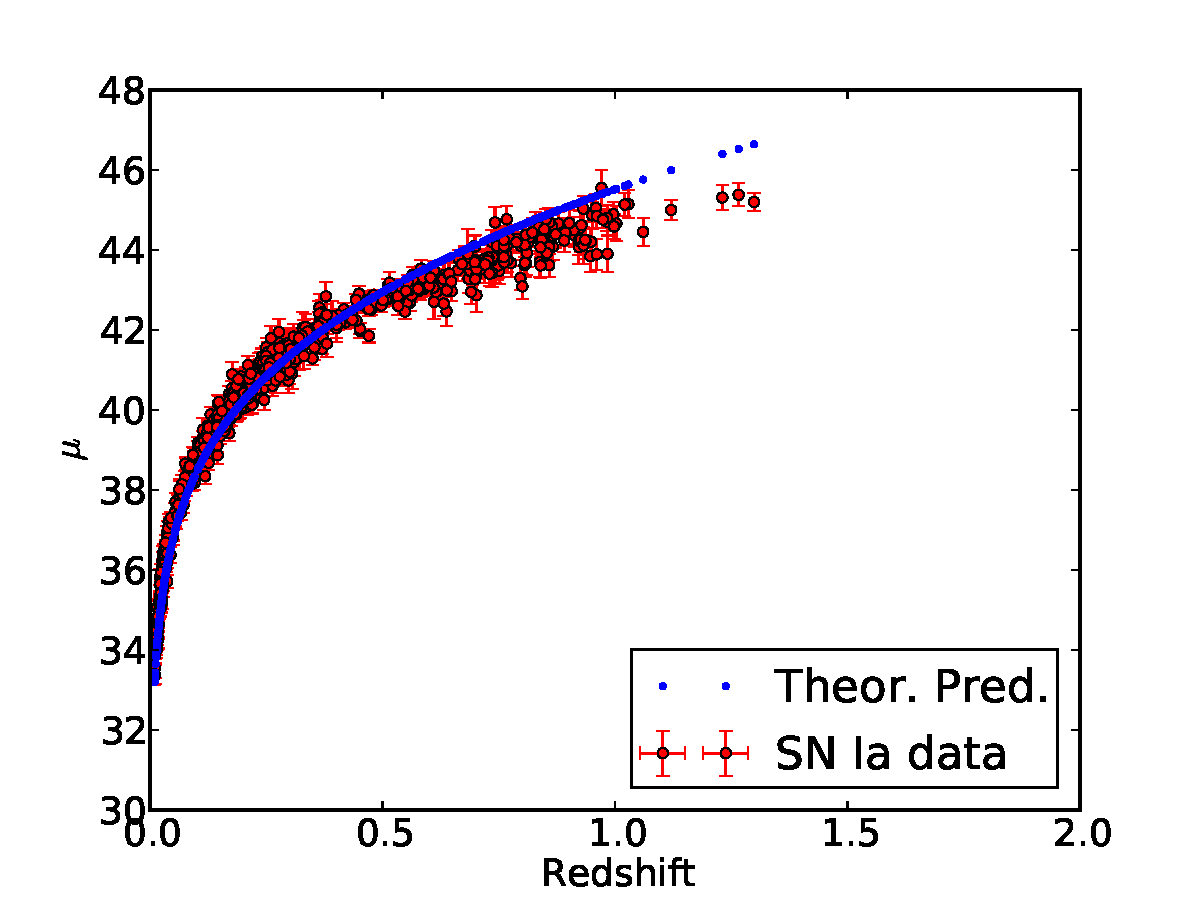
\includegraphics[width=0.5\textwidth]{../plots/mu.pdf}
\caption{\label{fig:mu}The distribution of distance modulii versus redshift for the SN Ia points used in the analysis from the JLA catalog. The $\mu_\text{model}$ distribution predicted by our best-fit value of $\Omega_l$, $\Omega_m$ is overlaid in blue.}
\end{figure}


\section{V. Discussion}
Our approach follows the steps of \cite{sdss}, using the same likelihood function and fit parameters but does not recover similar results. Areas of concern that may have negatively affected the results are the bounds on the parameters metioned in table 1, the jumping functions in the MCMC, and the method of finding the quoted values.

The ranges we let the parameter values explore was chosen such that they were centered around the results of \cite{sdss} as we expected the results to converge to answers similar to those. However from the trace plots and histgrams it is apparent that, while the distributions for $\alpha$ and $\Delta_m$ look good (approoximately normal distributions), it seems that $\beta$ and $\Delta_m$ could be allowed larger renges. One way we could have allowed for this was not choosing truncated gaussians as the distributions for drawming new parameter values. Furthermore, the histogram distributions for $\beta$ and $\Delta_m$ could perhaps be made to approximate tighter normal distribution by choosing a smaller a $\sigma < .6$ as not all the parameters need the same jumping distribution. 
For $\Omega_m$ a jumping distribution that is strictly between 0 and 1 is required since $\Omega_m$ cannot take values outside this range. As was discussed with $\beta$ and $\Delta_m$, a distribution with a sharper peak may have be achievable but decreasing the $\sigma$ of the jumping distrbution. The amount by which we should change these values for more acurate result would also require hand tunning as decreasing the variance of the jumping distributions can also cause the convergence process to take longer. Like before we would want to try to find a set of values that the acceptance rate of the newly drawn parameters at each step in the MCMC is between 30 and 70 \% \cite{MC}.

Not wanting to make to many assumptions about the shapes of our histograms we reported the median and average values. Another way to conclude the most favorable values of $\alpha$, $\beta$, $M'$, $Delta_m$, and $\Omega_m$, would be to fit the histograms to some distribution (e.g. a noral distribution, or a sum of two normal distributions) and report the values as the peaks and confidence levels given by the fit. This would, for example, given us a  higher value for $\beta$ because it appears $\beta$ is not able to explore its full range given our bounds.

Additionally, J.T. Nielson et al bring up concerns with the validity of using a $\chi^2$ likelihood distribution to evaluate the probability of different model parameter values. In future studies, to make a direct comparison with J.T. Nielson et al., our approach can be expanded to adopt their likelihood function. 
They employ an alternative likelihood function, which they define as \begin{align*}\mathscr{L} = |2\pi(C+A^T \Sigma_l A)|^{-1/2}\; \\
\times \text{Exp}[-(\hat{Z}-Y_0A)(C+A^T\Sigma_lA)^{-1}(\hat{Z}-Y_0A)^T/2],\end{align*} where $\Sigma_l = \text{diag}[\sigma_{M_0}^2,\sigma_{X_{1,0}}^2,\sigma_{C_0}^2,...],$ $A = ,$ $\hat{Z} = [\hat{m}_{B1}-\mu_1, \hat{x}_{11},\hat{c}_1,..]$, and $Y_0 = [M_0,x_{1,0},c_0,....]$. 
\par To make a more accurate comparison, this likelihood function should be implemented and compared directly to the $\chi^2$ likelihood function. Then, the authors' reported effect of the alternative likelihood measure could be accurately evaluated while keeping all of the other conditions (such as the host stellar mass handling) the same. 

\subsection{An unexplained peculiarity}
In trying to diagnoise problems with our MCMC, we came accross a peculiar phenomenon we thought worth breifly mentioning. Plotting the $\chi^2$ values verse $\Omega_M$ of the aggrigated data in \cref{fig:chi2}, $\chi^2$ never dips bellow about 2 for all values of $\Omega_M$. This seems to point towards our MCMC never quite being optimized by any of the sets of parameter values it draws. It is not apparent if this problem can be alleviated by the aforementioned changes. 

\begin{figure}
% %\centering
 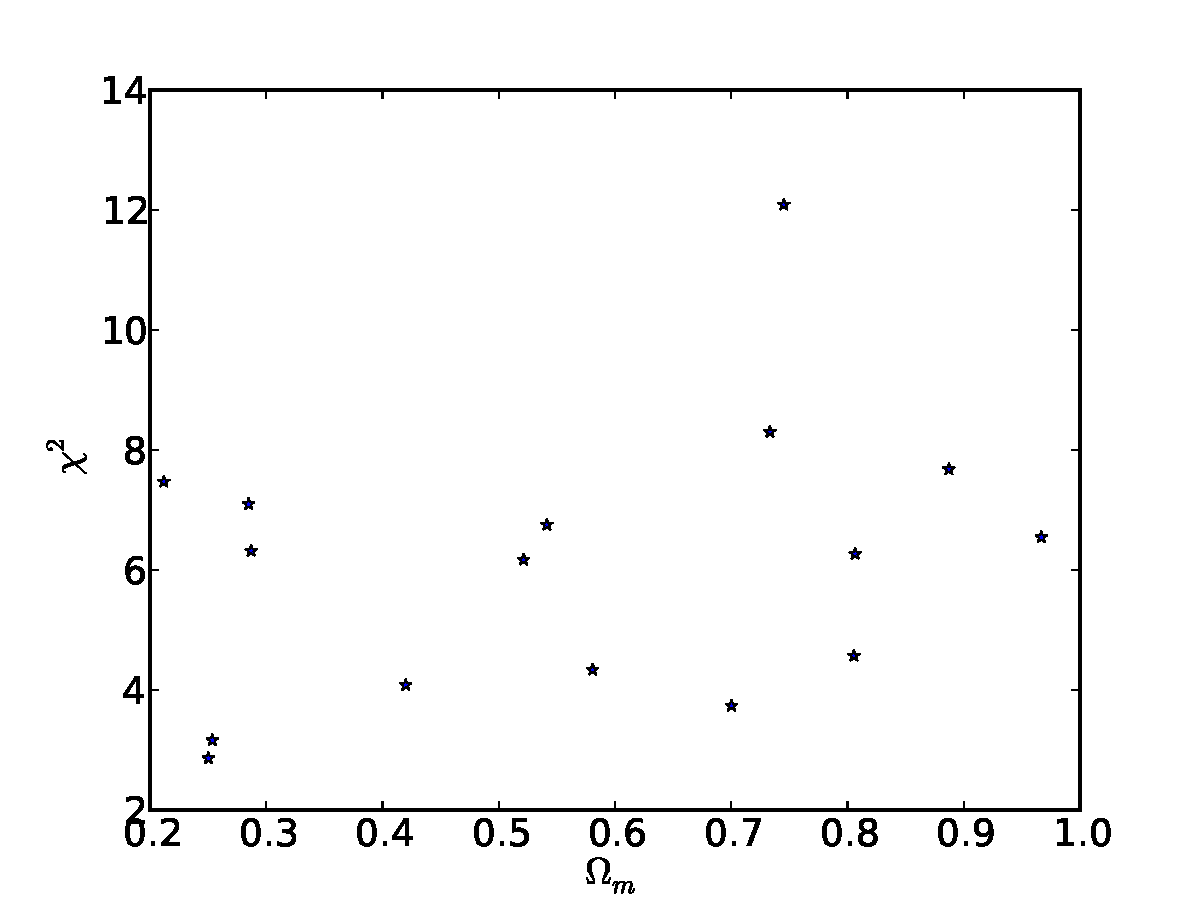
\includegraphics[width=0.5\textwidth]{../plots/om_chi.pdf}
\caption{\label{fig:chi2}The values of $\Omega_M$ from each MCMC versus the corresponding $\chi^2$ values.}
\end{figure}
 
\bibliographystyle{apsrev4-1} % Tell bibtex which bibliography style to use
\bibliography{cosmo_bib} 
\end{document}
